\section{Experimentación}

Para las diferentes mediciones necesarias para los experimentos presentados a continuación fueron realizadas sobre una CPU Intel 5200U en un sistema con 8GB de memoria RAM. Los binarios fueron compilados por \texttt{gcc 6.2.1 20160830} utilizando los flags \texttt{-O3 -std=c++11 -march=native}. El toolchain utilizado para correr las mediciones y realizar los gráficos puede encontrarse junto al código en \texttt{tools/data_analisis}.

Para las mediciones de tiempos se corre repetidamente el mismo problema no menos de 4 veces y 100ms para caso, y luego se almacena la media de las mediciones.

\subsection{Runtime de los algoritmos exactos}

En la figura \ref{fig:time-exacto} comparamos el tiempo de ejecución del algoritmo exacto de fuerza bruta con el de backtracking.
Para ello medimos con ambos 5 casos distintos para cada combinación de cantidad de gimnasios y paradas entre 2 y 5. Además usamos siempre un tamaño de mochila mayor a tres veces la cantidad de paradas.

\begin{figure}[H]
	\centering
	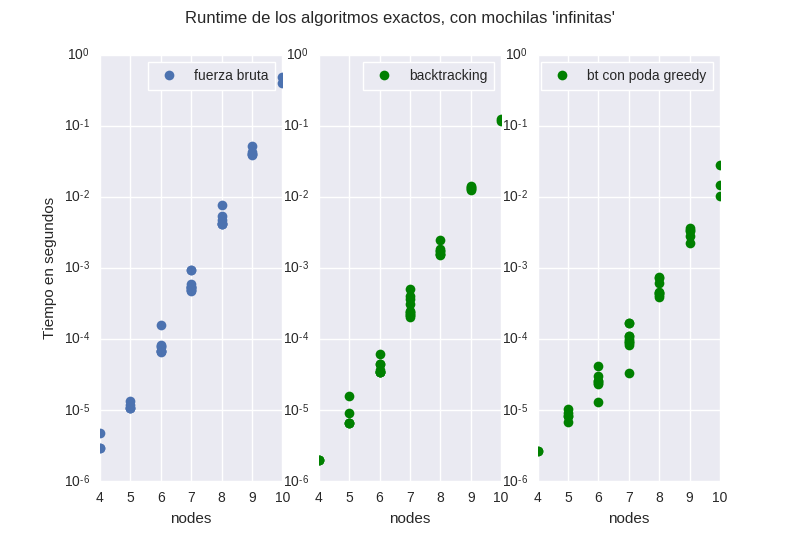
\includegraphics[width=\textwidth]{time-exacto}
	\caption{Tiempo de ejecución de algoritmos algoritmos exactos}
	\label{fig:time-exacto}
\end{figure}

Como podemos observar, ambos se comportan exponencialmente pero el backtracking resulta ser cerca de un orden de magnitud mas rápido.
\\

A continuación realizamos pruebas fijando la cantidad de gimnasios y paradas en 5 y variando el tamaño de la mochila.
Desafortunadamente vemos en la figura \ref{fig:time-exacto-moch} que dentro del intervalo de tamaños de mochila
interesantes, limitado por la cantidad de nodos que puede tener un problema a ser resuelto en un tiempo factible
(ya que si el tamaño es mayor a tres veces la cantidad de paradas, no influirá en el comportamiento del algoritmo),
no podemos determinar propiamente el comportamiento.

\begin{figure}[H]
	\centering
	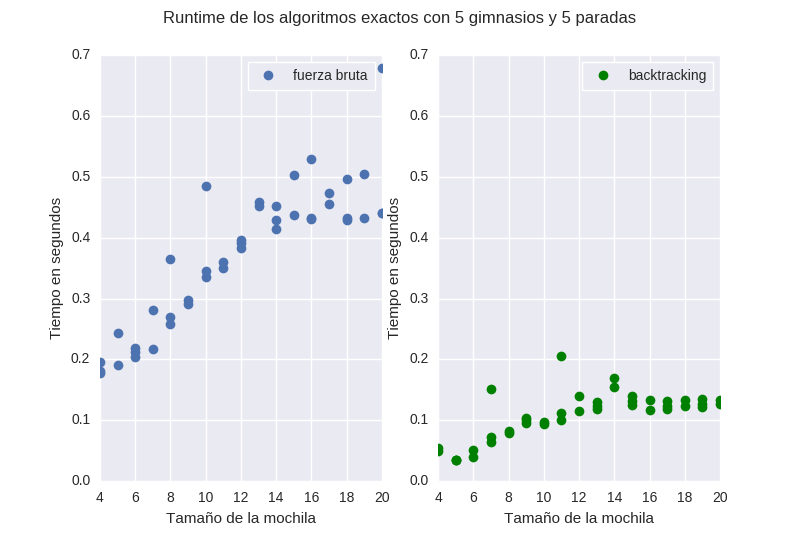
\includegraphics[width=\textwidth]{time-exacto-moch}
	\caption{Tiempo de ejecución de algoritmos algoritmos exactos al variar el tamaño de la mochila}
	\label{fig:time-exacto-moch}
\end{figure}

